\section{Beams}\label{sec:beam}

Once an array and element(s) have been defined, the user can generate any number of beam patterns by defining a set of wavelength-dependent, complex weights, $w(\lambda)$. Multiple beams can be calculated for the same array by changing these weights. The beam structure must contain these weights in a single field called \texttt{.ew}, which is a column vector of length \texttt{Array.Ne}.

In conventional (plane wave) beamforming, amplitude weights are used to adjust the width of the beam's main lobe and the magnitude of its sidelobes, and phase weights are used to steer the beam in azimuth and elevation. For a source in the array's acoustic near field, phase weights can also be used to focus the beam at a specified range. In adaptive beamforming, a complex set of weights is chosen to simultaneously maximize one criterion (e.g. signal level) and minimize one or more other criteria (e.g. noise level). Although the details of near-field focusing and adaptive beamforming are beyond the scope of this user's guide, Sonar Workbench can generate beam patterns for any complex weights the user derives.

\subsection{Conventional beamforming}

Conventional beamforming independently calculates amplitudes, $a_i$, and phases, $\phi_i$ to create complex weights $w_i=a_ie^{j\phi_i}$. Listing~\ref{lst:SampleBeam} shows an example of one beam that can be formed for the planar array example from Section~\ref{sec:array}. This example contains both amplitude and phase weights.

\lstinputlisting[caption={\texttt{SampleBeam.m}},label={lst:SampleBeam}]{../../examples/SampleBeam.m}

\subsubsection{Amplitude weights}

Amplitude shading exploits the Fourier transform relationship between the beam's aperture function and its far field beam pattern. Consequently, sonar designers often use weights, or shading coefficients, taken from standard window functions. Examples include Uniform, Hanning, Hamming, and Chebyshev, as shown in \figname~\ref{fig:WindowFunctions}. The example beamformer uses two Chebyshev windows, one of length 5 in the horizontal direction, and one of length 10 in the vertical direction. The total weight for each element is the product of the two windows evaluated at its coordinate the horizontal and vertical direction.

\begin{figure}[!ht]
\begin{center}
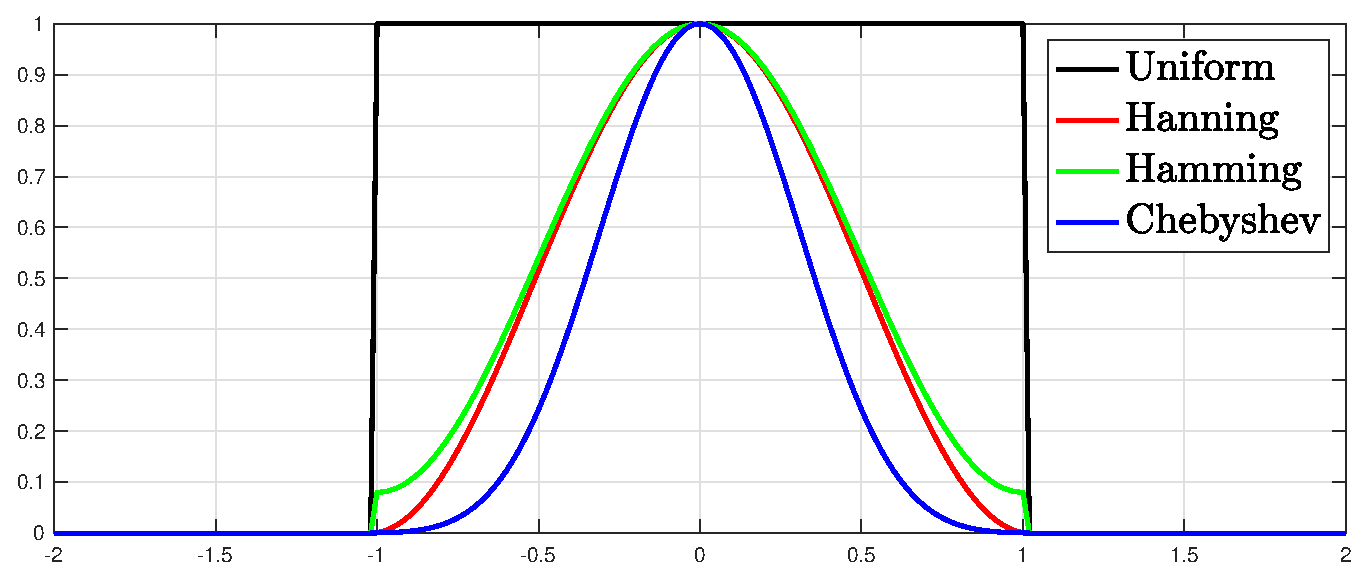
\includegraphics[width=\textwidth]{WindowFunctions}
\caption{\label{fig:WindowFunctions}Common window functions used for amplitude shading}
\end{center}
\end{figure}

Since the final beam pattern will be normalized for unity gain along its maximum response axis, the user is not required to normalize the amplitude weights or limit their amplitude. However, it is best to avoid negative amplitude weights and instead represent negative numbers with phase weights.

\subsubsection{Phase weights}

Without phase weights, i.e. the beam pattern weights are purely real, the beam pattern is unsteered. The user can steer the beam to an arbitrary elevation and azimuth, ($\theta_0$,$\psi_0$) using the following formula for the $i^{th}$ element's phase,
\begin{equation}
\phi_i(\lambda,\theta_0,\psi_0) = -2\pi\left(\frac{\cos\theta_0\cos\psi_0}{\lambda}x_i + \frac{\cos\theta_0\sin\psi_0}{\lambda}y_i + \frac{\sin\theta_0}{\lambda}z_i \right).
\end{equation}
